\documentclass[11pt]{article}
\usepackage[margin=0.8in]{geometry}
\usepackage{amsmath,amssymb,graphicx,tabularx,booktabs,xcolor}
\usepackage[colorlinks=true,urlcolor=blue]{hyperref}
\setlength{\parindent}{0pt}\setlength{\parskip}{7pt}
\setlength{\emergencystretch}{2em}
\newcommand{\Pbase}{/home/ec2-user/pencil-controller-review-20261029/c1-takeover-20261030}
\newcommand{\Hbase}{/home/ec2-user/crypto-pr2304-persist/research}
\newcommand{\Cbase}{/home/ec2-user/crypto-pencil-signed-graph-20261029/research}
\begin{document}
{\LARGE Four-lead reconciliation packet}\par
{\large Source-linked mathematics, archived evidence and software qualification}\par
2026-10-30 UTC. Snapshot time is recorded in \texttt{snapshot-utc.txt}.

\textbf{Completed components.} The evidence index preserves the four research leads' existing target rows, cost grids and reports. A written same-support derivation connects valid-input polynomial divisibility to two coefficient identities used by the runtime classifier. The diagnostics, lifecycle, owner and campaign-accounting implementation has software-test and static-build receipts. This packet makes those components inspectable together.

\textbf{Archive coverage.} The counts below are transcribed from the retained inventory and reports; they are not fresh experimental runs. Arm repetitions are not additional distinct targets.

\begin{tabularx}{\textwidth}{@{}p{0.19\textwidth}X@{}}\toprule
Lead & Preserved evidence and scope\\\midrule
Factor-base / graph & Five arms (\texttt{full\_8}, \texttt{full\_16}, \texttt{full\_32}, \texttt{half\_16}, \texttt{quarter\_16}), each 1,260 distinct workload IDs; 6,300 rows tagged \texttt{priced\_source\_verified}. A further partial-relation graph-policy sweep is prospective.\\
Weighted genus-2 law & Wrapper and retained-state arms each have 1,260 archived targets. Source audits, replay certificates and pricing grids are preserved. Split-normalization inversions remain charged in the retained-state accounting.\\
Pencil collector & Historical shared index: 543 distinct workloads with a verified candidate, one capped-only, 716 unindexed. Later C1 terminal packet: 7/18 executions, 4/15 measured, two candidate timeouts, zero successful candidate/reference pairs and 36 null ratio cells.\\
Kummer & Differential uncached archive: 1,260 paired indexed rows. Separate N19 labelled fallback archive: 1,260 verified candidate/baseline/rho targets and zero observed fallback steps. The separate 1,260-row coordinate gate is not a collector run.\\\bottomrule
\end{tabularx}

\textbf{Review inputs.} The shared historical target table has 12,850 rows and its cost table has 3,067 rows in the retained inventory. N19 has separate tables. Their heterogeneous arms and boundaries should be inspected before comparisons; this packet adds no pooled estimate or cost ratio. Existing PDFs and grids are linked on page 4, with full paths and hashes in \texttt{artifact-index.json}.

\newpage
{\Large Same-support branch: bounded mathematical derivation}

\textbf{Domain.} Work over a field $K$. Both inputs have nonzero $z_i,w_i$, normalize to the same monic quadratic $u$, and satisfy $u\mid f-v_i^2$ for the same polynomial $f$, with $v_i=\bar s_iX+\bar t_i$ and $\bar s_1=\bar s_2$. The source normalization is
\[
\bar q_i=q_i/z_i^2,\quad \bar r_i=r_i/z_i^4,\quad
\bar s_i=s_i/(z_i^3w_i),\quad \bar t_i=t_i/(z_i^5w_i).
\]
Subtracting the valid-input divisibilities gives $u\mid D=v_2^2-v_1^2$. Equal slopes cancel the quadratic term, leaving
\[
D=(\bar t_2-\bar t_1)(\bar s_1+\bar s_2)X
 +(\bar t_2-\bar t_1)(\bar t_2+\bar t_1).
\]
Because $u$ is monic of degree two and $D$ has degree at most one, $D=0$. Its two coefficients therefore vanish.

\textbf{Connection to literal runtime expressions.} Let $Z=z_1z_2$ and $W=w_1w_2$. The cross-scaled source expressions satisfy
\[
Q_{ci}=Z^2\bar q_i,\quad R_{ci}=Z^4\bar r_i,\quad
S_{ci}=Z^3W\bar s_i,\quad T_{ci}=Z^5W\bar t_i.
\]
Multiplying the coefficient identities by $Z^8W^2$ and $Z^{10}W^2$ yields
\[
(T_{c2}-T_{c1})(S_{c1}+S_{c2})=0,\qquad
(T_{c2}-T_{c1})(T_{c2}+T_{c1})=0.
\]
These supply the coefficient hypotheses of the existing abstract same-support classifier. Its odd-characteristic condition is additional to the polynomial implication. With those conditions, the proposed connection excludes the mixed zero-slope branch after the classifier's order of inverse and equality checks.

\textbf{Checks and next dependency.} The written derivation and nonblind source feedback cover this bounded scaling argument. A Lean draft exists; the pinned helper import exceeded a 120-second cap while waiting on RPC-backed dependency access. The candidate module was not reached, no new theorem axiom output was produced, and the owned processes were reaped. The next technical check is that exact draft under a functioning pinned dependency cache, followed by the compiled-source invariant and branch connection. Universal addition-law completeness also needs the remaining branch and divisor-class obligations.

Sources: \href{\Pbase/four-lead-inventory-resume/same-support-derivation.md}{derivation}, \href{\Pbase/four-lead-inventory-resume/same-support-independent-review.md}{nonblind feedback}, \href{\Pbase/four-lead-inventory-resume/lean-candidate/qualification-receipt.json}{bounded Lean attempt receipt}, \href{\Pbase/four-lead-inventory-resume/law-remaining-obligations.md}{remaining obligations}. Literal Rust locations and source hashes are in \texttt{law-source-hashes.json}.

\newpage
{\Large Implementation and software qualification}

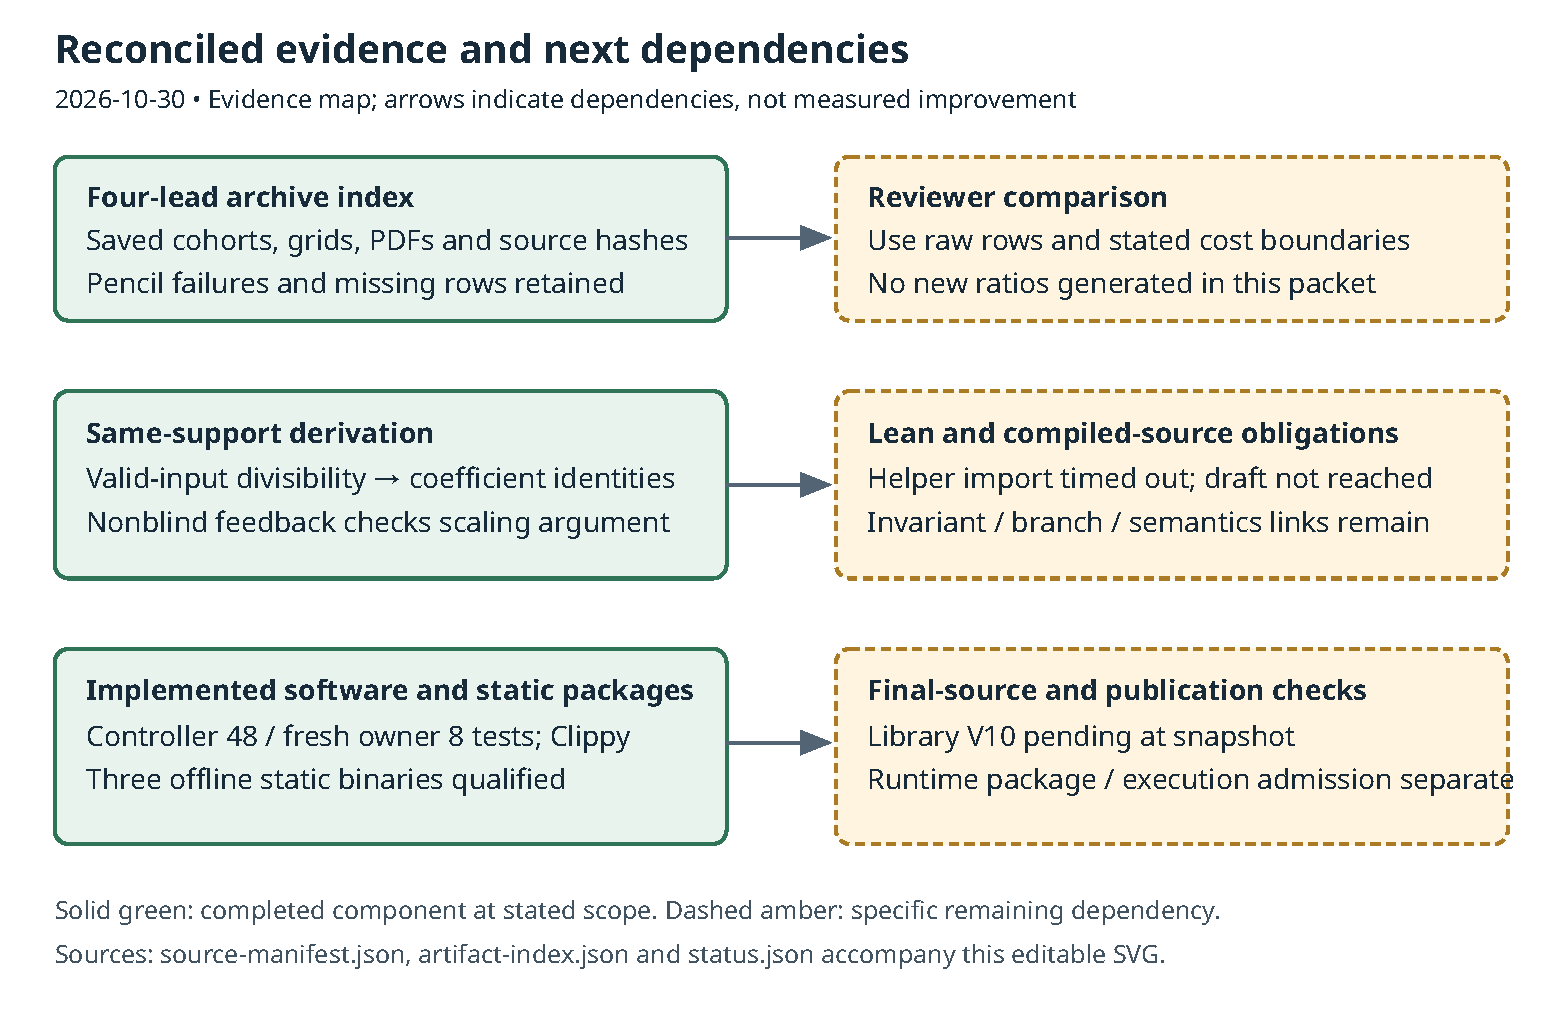
\includegraphics[width=\textwidth]{dependencies.pdf}

\begin{tabularx}{\textwidth}{@{}p{0.25\textwidth}X@{}}\toprule
Component & Recorded qualification\\\midrule
Library V8 & Earlier source: 5,660 passed, zero failed, 124 ignored. Final-source V10 remains pending at this snapshot.\\
Controller V5 & 48 software tests passed; strict Clippy passed.\\
Fresh owner V4 & Six unit and two integration tests passed; strict Clippy passed.\\
Static packages & Controller, progress and fresh-owner binaries built offline for x86-64 musl with Rust 1.99.1; ELF checks found no interpreter or dynamic dependencies. These binary artifacts were not executed in the qualification.\\\bottomrule
\end{tabularx}

The implementation carries explicit launch context, bounded diagnostic sidecars, owner receipts, absolute/monotonic cutoffs and conservative campaign admission. Source manifests bind each check to its actual corpus. Static package qualification is separate from a published runtime image and its execution checks. Conservative allocation reservations are not measured worker costs.

No new scientific execution or cloud publication accompanies this report. The recorded campaign limits remain 25,200 cumulative seconds and the absolute deadline 2026-10-30 22:08:40 UTC. No interval or allowance is reset by this reconciliation.

\newpage
{\Large Evidence index and reviewer entry points}

\begin{enumerate}
\item \href{\Hbase/four_followups_review_20261022/REPORT.pdf}{Shared four-followup report}; \href{\Hbase/four_followups_review_20261022/results/standard-targets.csv}{standard target rows}; \href{\Hbase/four_followups_review_20261022/results/standard-cost-grid.csv}{standard cost grid}. Use workload IDs to distinguish repeated arms.
\item \href{\Hbase/four_followups_20261021/results/matched/price-grid.csv}{Factor-base matched price grid}. Compare the five named arms under the archived pricing definitions.
\item \href{\Hbase/projective_law_followup_20261022/REPORT.pdf}{Weighted-law report}; \href{\Hbase/projective_law_followup_20261022/results/price-grid-projective.csv}{wrapper price grid}; \href{\Hbase/projective_law_followup_20261022/results/price-grid-state.csv}{retained-state price grid}. Finite audit coverage and universal compiled semantics are separate entries.
\item \href{\Cbase/pencil_large_prime_20261029/validation/accounting/reports/run-20261030T0543Z-c1-terminal/review-packet.pdf}{C1 terminal pencil packet}; \href{\Cbase/pencil_large_prime_20261029/validation/accounting/reports/run-20261030T0543Z-c1-terminal/cost-grid-exact.csv}{exact terminal grid}. Preserve null ratio cells and timeout rows. Terminal completeness findings and unperformed independent terminal replay remain recorded.
\item \href{\Hbase/kummer_differential_collector_20261022/KUMMER_PAIRED.pdf}{Paired Kummer report}; \href{\Hbase/kummer_differential_collector_20261022/n19-labelled-fallback/REPORT.pdf}{N19 fallback report}; \href{\Hbase/kummer_differential_collector_20261022/n19-labelled-fallback/results/analysis/price-grid.csv}{N19 grid}. Zero naturally observed fallback steps differs from the forced-zero fixture coverage.
\item \href{\Pbase/controller-progress-static-qualification-v1/QUALIFICATION.json}{Controller/progress static qualification}; \href{\Pbase/fresh-owner-static-qualification-v2/BUILD-RECEIPT.json}{final fresh-owner static build receipt}. These identify exact binaries and their source corpus.
\end{enumerate}

\textbf{Standardized packet files.} \texttt{status.json} retains machine-readable status rows and count provenance; \texttt{artifact-index.json} links archived reports/grids with recorded hashes; \texttt{source-manifest.json} hashes the evidence used here. \texttt{dependencies.svg} is the editable diagram source. \texttt{report.tex} and \texttt{create-packet.sh} preserve report generation and index extraction. The PDF's links point to local preserved artifacts, so reviewers need access to those paths or an equivalent archive.

\textbf{Review method.} This is a derived reconciliation, using the existing inventory, written algebra, source feedback and immutable software receipts. It does not repeat target arithmetic, revise historical measurements, or add a statistical interpretation. Pending status is time-stamped; a later completed check should be published as an additive packet update with its own exact receipt.
\end{document}
